\documentclass[11pt,table]{article}
\usepackage{lmodern}
\usepackage{amssymb,amsmath}
\usepackage{ifxetex,ifluatex}
\usepackage{fixltx2e} % provides \textsubscript
\ifnum 0\ifxetex 1\fi\ifluatex 1\fi=0 % if pdftex
  \usepackage[T1]{fontenc}
  \usepackage[utf8]{inputenc}
\else % if luatex or xelatex
  \ifxetex
    \usepackage{mathspec}
  \else
    \usepackage{fontspec}
  \fi
  \defaultfontfeatures{Ligatures=TeX,Scale=MatchLowercase}
    \setmainfont[]{Georgia}
\fi
% use upquote if available, for straight quotes in verbatim environments
\IfFileExists{upquote.sty}{\usepackage{upquote}}{}
% use microtype if available
\IfFileExists{microtype.sty}{%
\usepackage{microtype}
\UseMicrotypeSet[protrusion]{basicmath} % disable protrusion for tt fonts
}{}
\usepackage[margin=1.in]{geometry}
\usepackage{hyperref}
\hypersetup{unicode=true,
            pdfborder={0 0 0},
            breaklinks=true}
\urlstyle{same}  % don't use monospace font for urls
\usepackage{graphicx,grffile}
\makeatletter
\def\maxwidth{\ifdim\Gin@nat@width>\linewidth\linewidth\else\Gin@nat@width\fi}
\def\maxheight{\ifdim\Gin@nat@height>\textheight\textheight\else\Gin@nat@height\fi}
\makeatother
% Scale images if necessary, so that they will not overflow the page
% margins by default, and it is still possible to overwrite the defaults
% using explicit options in \includegraphics[width, height, ...]{}
\setkeys{Gin}{width=\maxwidth,height=\maxheight,keepaspectratio}
\IfFileExists{parskip.sty}{%
\usepackage{parskip}
}{% else
\setlength{\parindent}{0pt}
\setlength{\parskip}{6pt plus 2pt minus 1pt}
}
\setlength{\emergencystretch}{3em}  % prevent overfull lines
\providecommand{\tightlist}{%
  \setlength{\itemsep}{0pt}\setlength{\parskip}{0pt}}
\setcounter{secnumdepth}{5}
% Redefines (sub)paragraphs to behave more like sections
\ifx\paragraph\undefined\else
\let\oldparagraph\paragraph
\renewcommand{\paragraph}[1]{\oldparagraph{#1}\mbox{}}
\fi
\ifx\subparagraph\undefined\else
\let\oldsubparagraph\subparagraph
\renewcommand{\subparagraph}[1]{\oldsubparagraph{#1}\mbox{}}
\fi

%%% Use protect on footnotes to avoid problems with footnotes in titles
\let\rmarkdownfootnote\footnote%
\def\footnote{\protect\rmarkdownfootnote}

%%% Change title format to be more compact
\usepackage{titling}

% Create subtitle command for use in maketitle
\newcommand{\subtitle}[1]{
  \posttitle{
    \begin{center}\large#1\end{center}
    }
}

\setlength{\droptitle}{-2em}

  \title{}
    \pretitle{\vspace{\droptitle}}
  \posttitle{}
    \author{}
    \preauthor{}\postauthor{}
    \date{}
    \predate{}\postdate{}
  
\usepackage{booktabs}
\usepackage{longtable}
\usepackage{array}
\usepackage{multirow}
\usepackage[table]{xcolor}
\usepackage{wrapfig}
\usepackage{float}
\usepackage{colortbl}
\usepackage{pdflscape}
\usepackage{tabu}
\usepackage{threeparttable}
\usepackage[final]{changes}
\usepackage[font={small},labelfont=bf,labelsep=colon]{caption}
\linespread{2}
\usepackage{enumitem}
\usepackage{tikz}
\def\checkmark{\tikz\fill[scale=0.4](0,.35) -- (.25,0) -- (1,.7) -- (.25,.15) -- cycle;}
\setlist{nolistsep}
\setremarkmarkup{(#2)}

\begin{document}

\newpage

\begin{figure}
\centering
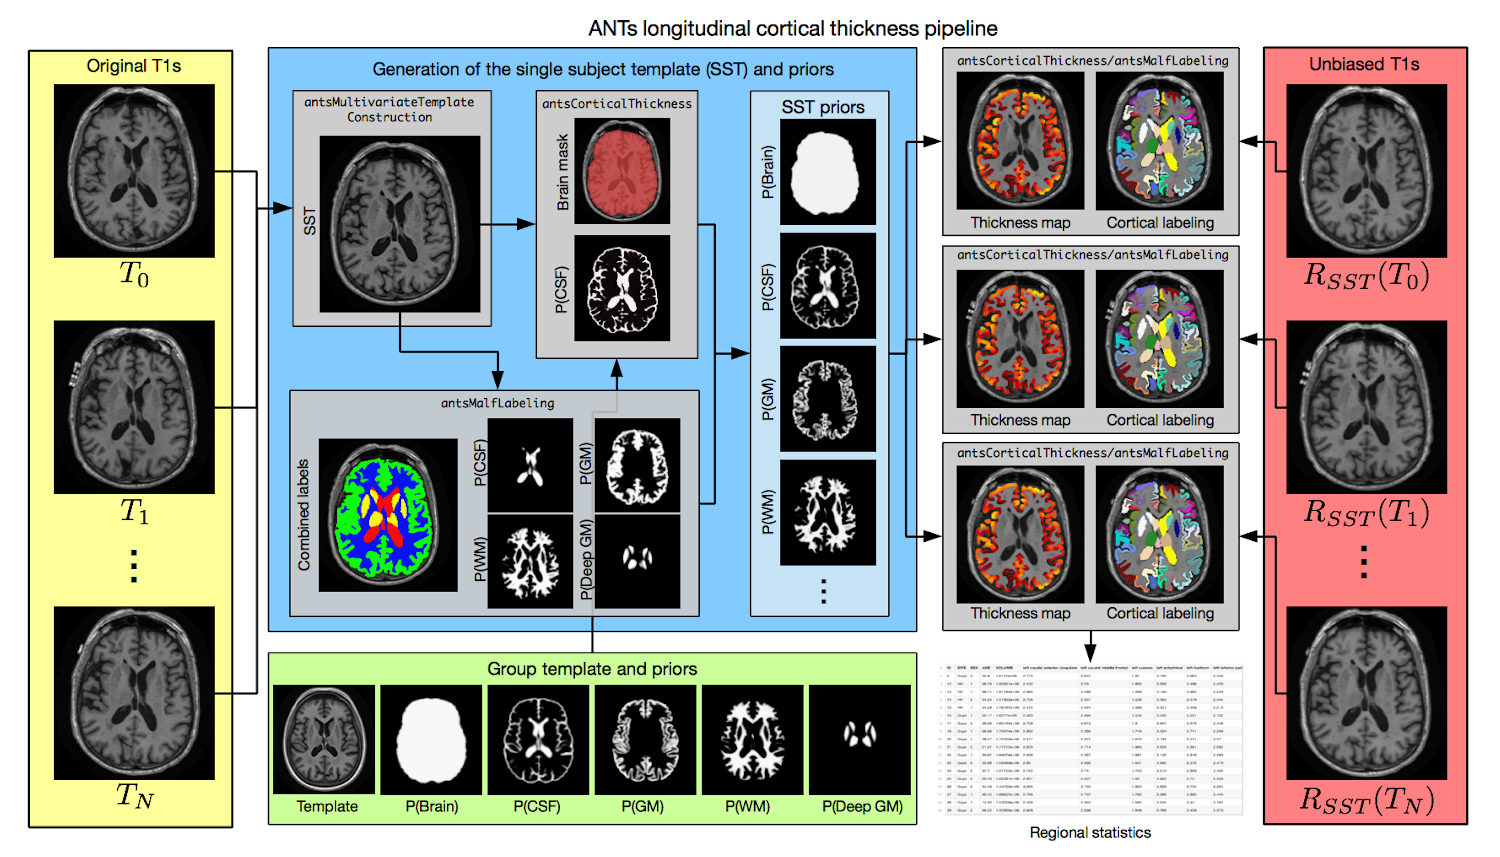
\includegraphics[width=\textwidth]{Figure3.pdf}
\caption{Diagrammatic illustration of the ANTs longitudinal cortical thickness pipeline
for a single subject with $N$ time points.  From the $N$ original T1-weighted
images (left column, yellow panel) and the group template and priors (bottom row,
green panel), the single-subject template (SST) and auxiliary prior images
are created (center, blue panel).  These subject-specific template and other
auxiliary images are used to generate the individual time-point cortical
thickness maps, in the individual time point's native space (denoted as
``ANTs Native'' in the text).  Optionally, one can
rigidly transform the time-point images prior to segmentation and cortical thickness
estimation (right column, red panel).  This alternative processing scheme is referred
to as ``ANTs SST''.  For regional thickness values, regional labels
are propagated to each image using a given atlas set (with cortical labels)
and joint label fusion.}
\label{fig:pipeline}
\end{figure}

\newpage

\begin{figure}
\centering
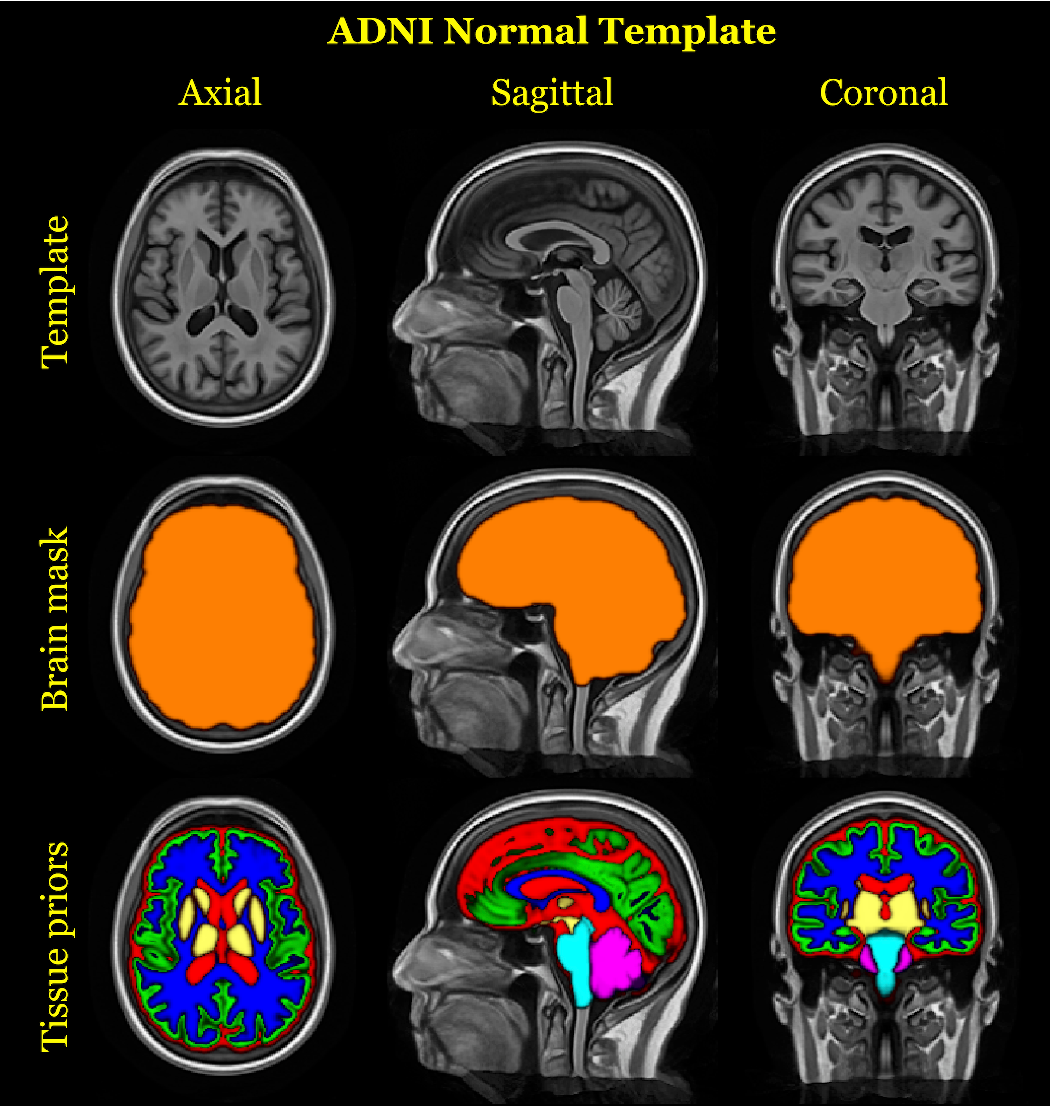
\includegraphics[width=\textwidth]{Figure4.pdf}
\caption{Top row:  Canonical views of the template created from 52 randomly selected
cognitively normal subjects
of the ADNI-1 database.  The prior probability mask for the whole brain (middle row)
and the six tissue priors (bottom row) are used to ``seed'' each single-subject template for creation of
a probabilistic brain mask and probabilistic tissues priors during longitudinal
processing.}
\label{fig:template}
\end{figure}

\newpage

\begin{figure}
\centering
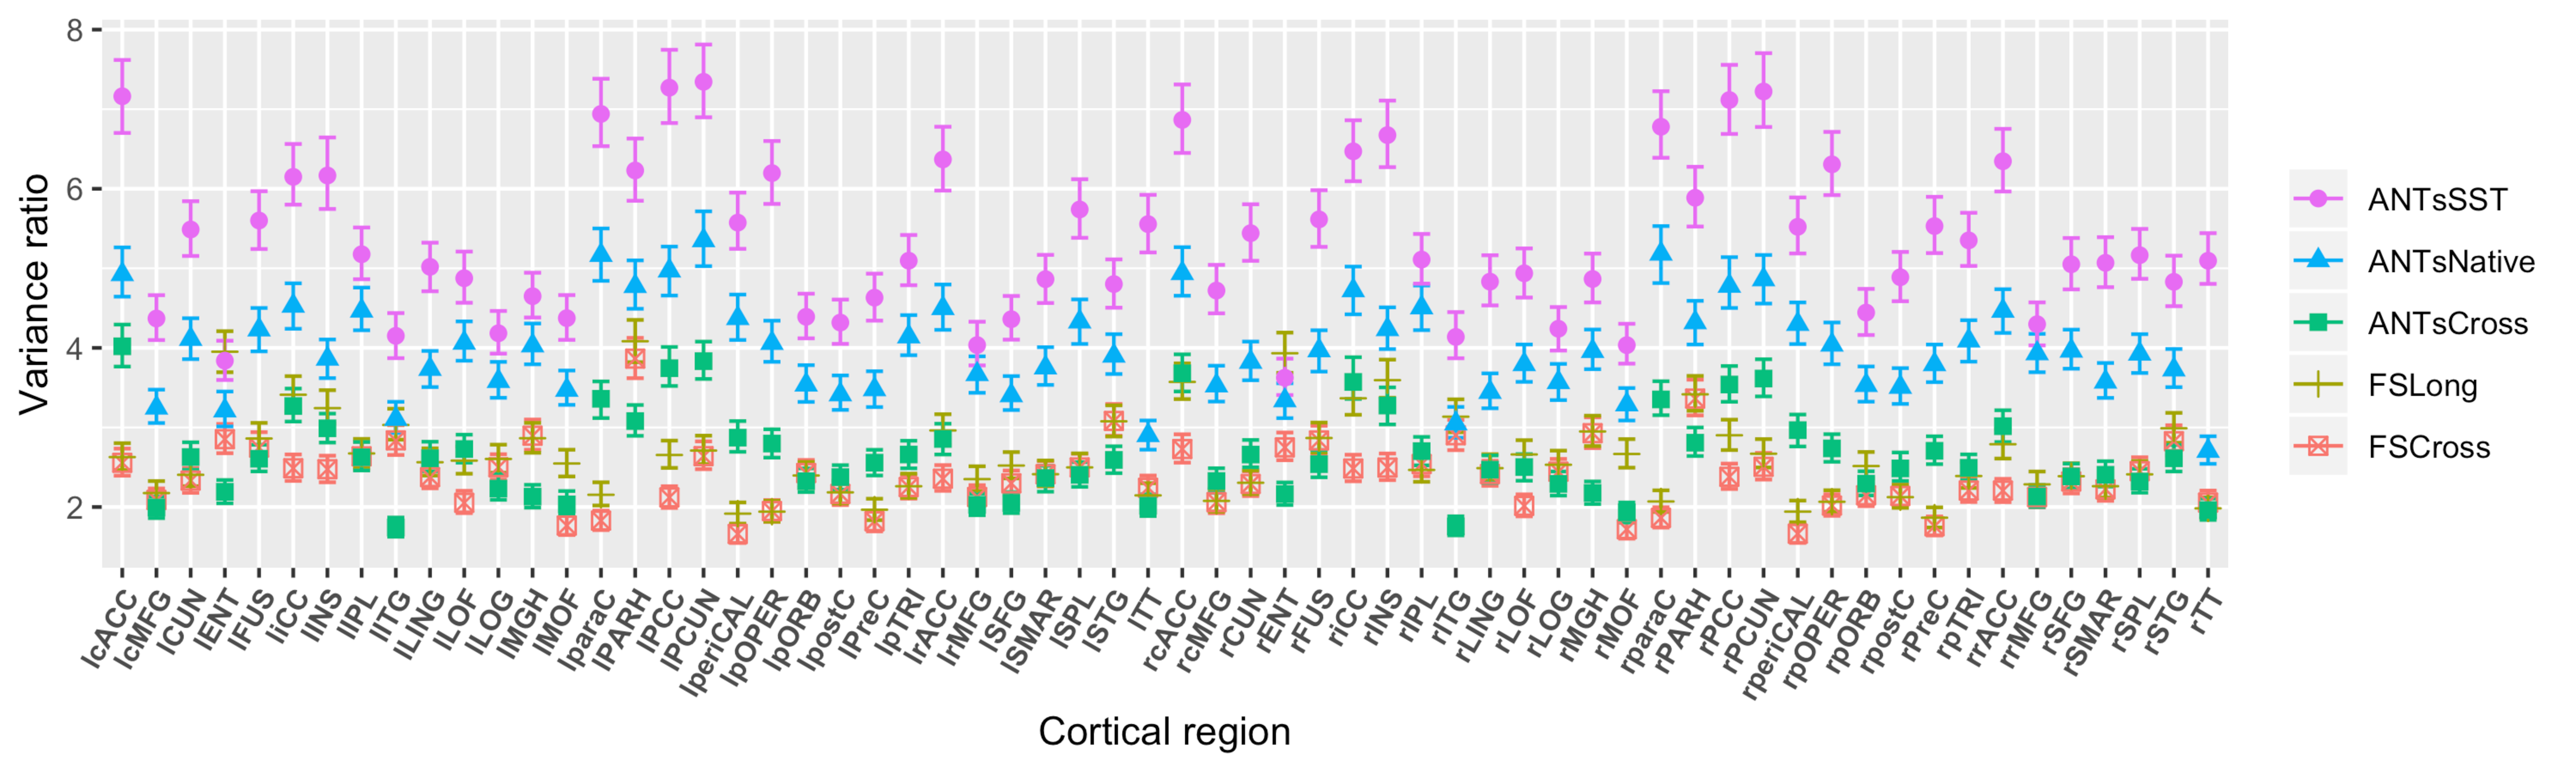
\includegraphics[width=\textwidth]{Figure6.pdf}
\caption{95\% credible intervals of the region-specific variance ratios
$r^k=\tau_k/\sigma_k$ are presented for each processing method.  The ANTs
SST method dominates the others across the majority of
regions---its point estimates (posterior medians) are greater than those of the other
processing methods except for the left and right EC values in
FreeSurfer Long (although there is significant overlap in the credible intervals
in those regions).
These results also suggest that longitudinal processing is to be
preferred for both packages.}
\label{fig:ratios}
\end{figure}

\clearpage
\newpage

\begin{figure}
\centering
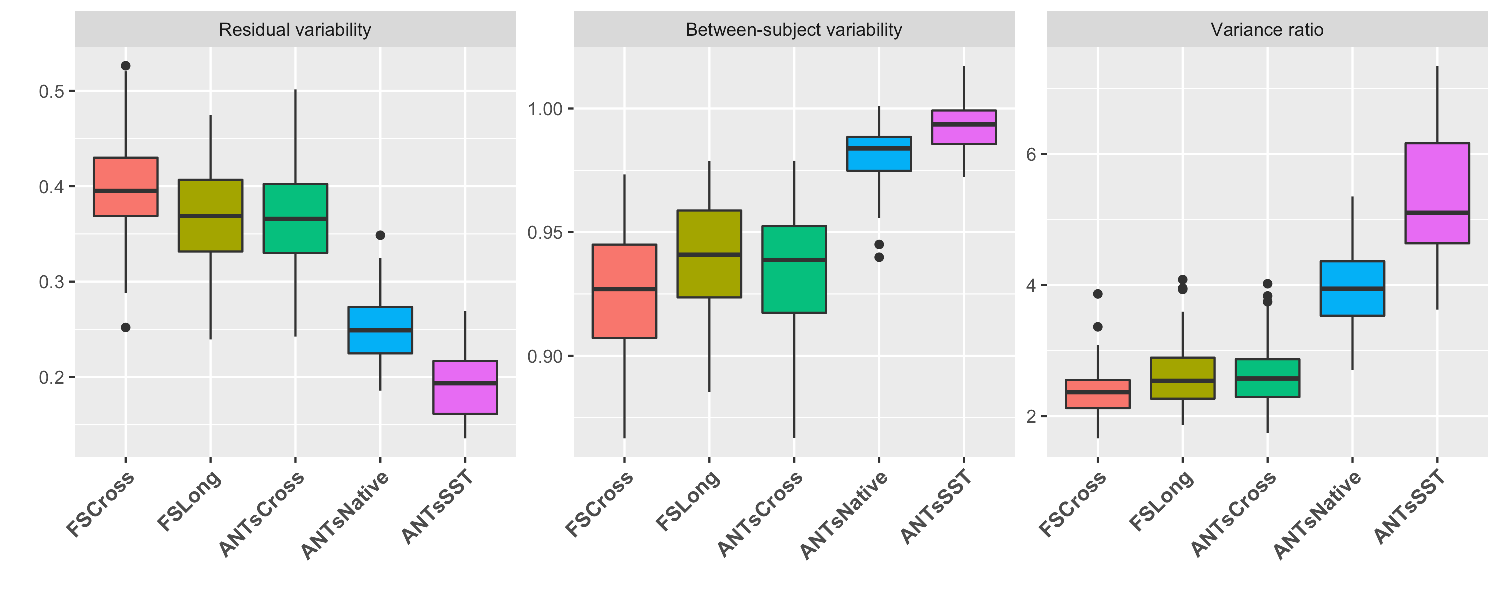
\includegraphics[width=\textwidth]{Figure7.pdf}
\caption{Box plots showing the distribution of the residual variability,
between subject variability, and ratio of the between-subject variability and
residual variability for each of the 62 DKT regions.  Note that the
``better'' measurement maximizes this latter ratio.}
\label{fig:variance_boxplots}
\end{figure}

\newpage

\begin{figure}
\centering
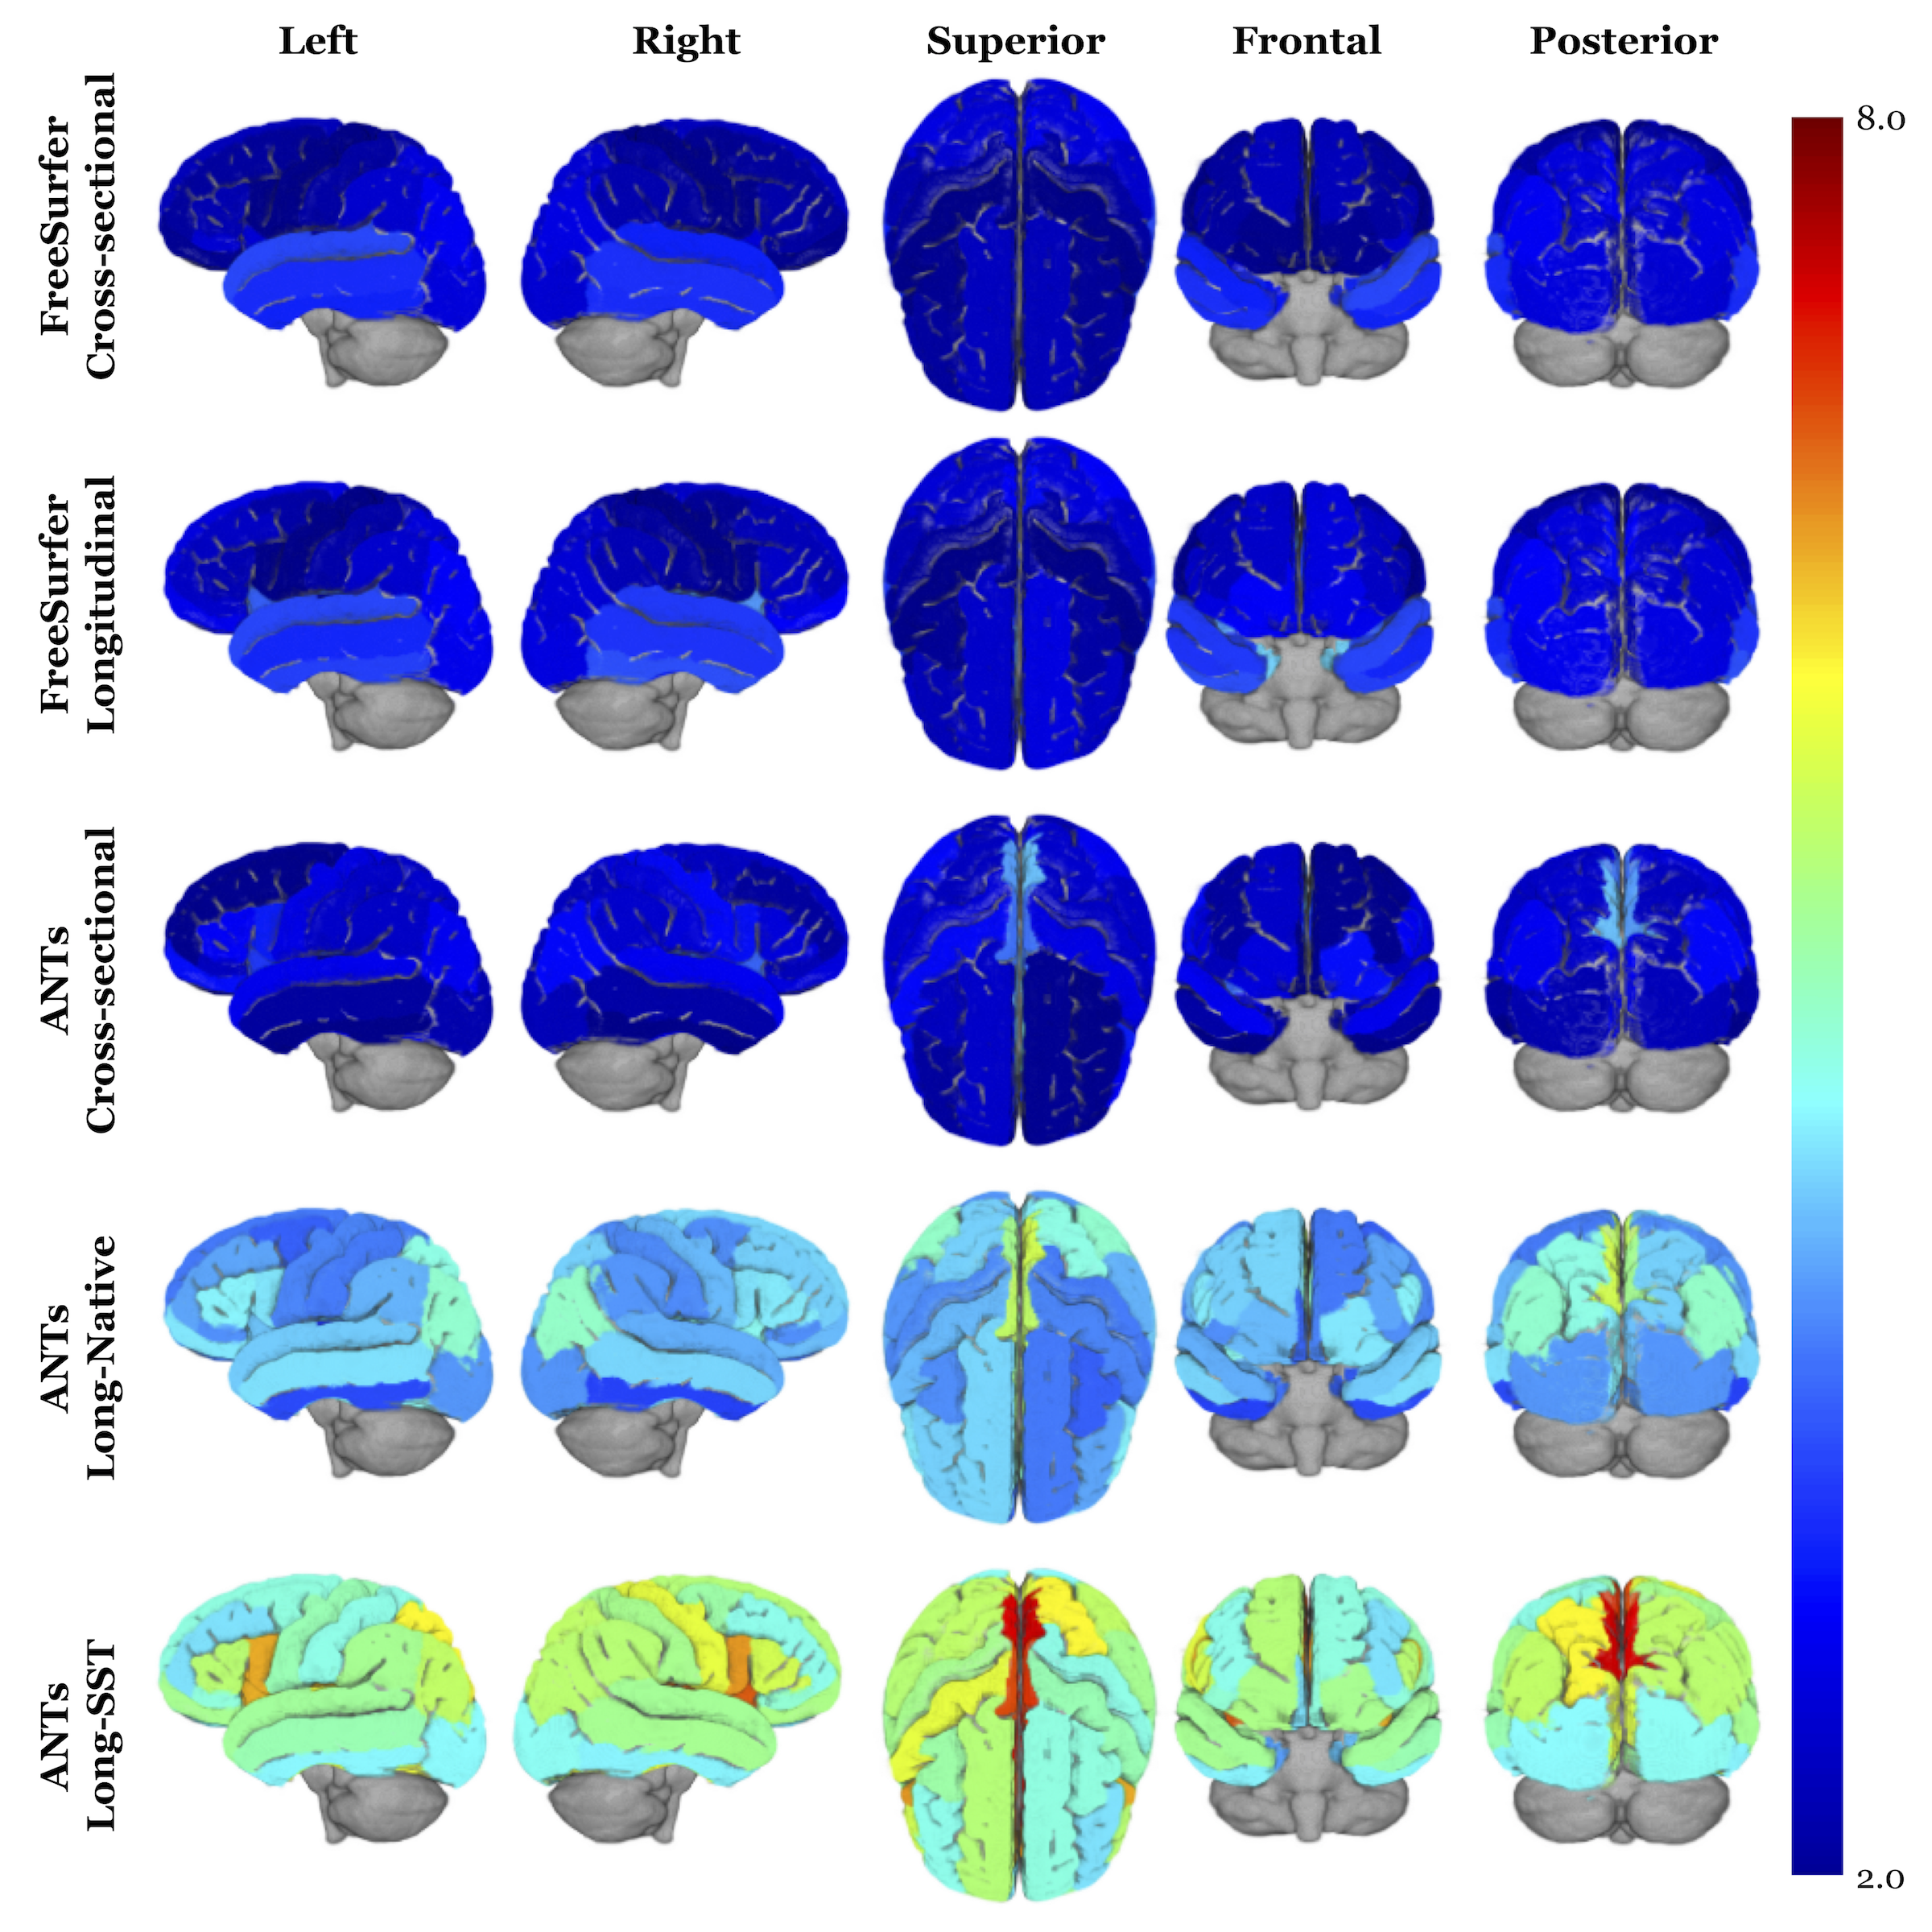
\includegraphics[width=\textwidth]{Figure8.pdf}
\caption{3-D volumetric rendering of the regional variance ratio values on the generated ADNI template.
The higher variance ratios indicate greater between-subject to residual variability.}
\label{fig:brain_variance}
\end{figure}

\newpage

\begin{figure}
\centering
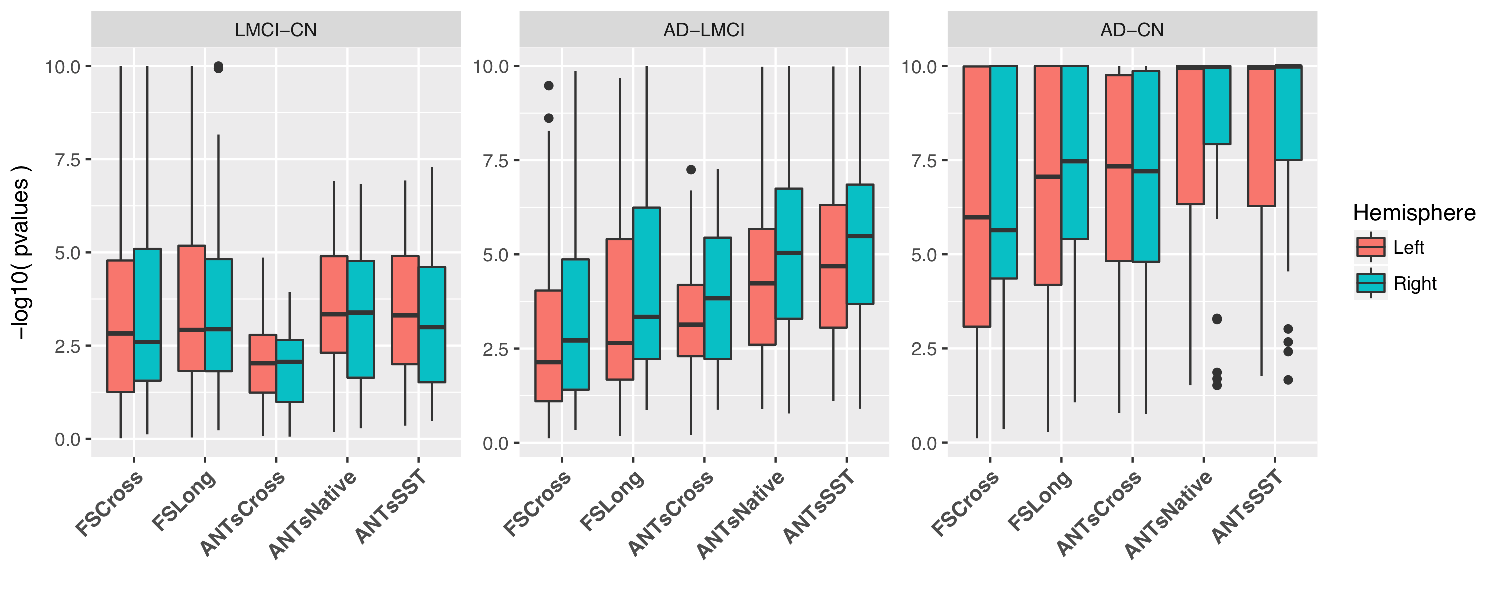
\includegraphics[width=1.0\textwidth]{Figure9.pdf}
\caption{
Log-scaled $p$-values summarizing Tables 2 and 3 demonstrating performance differences
across cross-sectional and longitudinal pipelines for the three diagnostic contrasts.
}
\label{fig:logpvalues}
\end{figure}

\newpage

%\documentclass{standalone}
%\usepackage{booktabs}
%\begin{document}
%\begin{tabular*}{1\textwidth}{@{\extracolsep{\fill}} l l}
%  \toprule
%  \midrule
%  1) caudal anterior cingulate ({\tt cACC})  & 17) pars orbitalis ({\tt pORB}) \\
%  2) caudal middle frontal ({\tt cMFG})      & 18) pars triangularis ({\tt pTRI}) \\
%  3) cuneus ({\tt CUN})                      & 19) pericalcarine ({\tt periCAL}) \\
%  4) entorhinal ({\tt ENT})                  & 20) postcentral ({\tt postC}) \\
%  5) fusiform ({\tt FUS})                    & 21) posterior cingulate ({\tt PCC}) \\
%  6) inferior parietal ({\tt IPL})           & 22) precentral ({\tt preC}) \\
%  7) inferior temporal ({\tt ITG})           & 23) precuneus ({\tt PCUN}) \\
%  8) isthmus cingulate ({\tt iCC})           & 24) rosterior anterior cingulate ({\tt rACC}) \\
%  9) lateral occipital ({\tt LOG})           & 25) rostral middle frontal ({\tt rMFG}) \\
%  10) lateral orbitofrontal ({\tt LOF})      & 26) superior frontal ({\tt SFG}) \\
%  11) lingual ({\tt LING})                   & 27) superior parietal ({\tt SPL}) \\
%  12) medial orbitofrontal ({\tt MOF})       & 28) superior temporal ({\tt STG}) \\
%  13) middle temporal ({\tt MTG})            & 29) supramarginal ({\tt SMAR}) \\
%  14) parahippocampal ({\tt PARH})           & 30) transverse temporal ({\tt TT}) \\
%  15) paracentral ({\tt paraC})              & 31) insula ({\tt INS}) \\
%  16) pars opercularis  ({\tt pOPER})        & {}\\
%  \bottomrule
%\end{tabular*}
%\end{document}


\begin{table}[!htb]
\centering
\caption{The 31 cortical labels (per hemisphere) of the Desikan-Killiany-Tourville atlas.
        The ROI abbreviations from the R {\tt brainGraph} package are given in
        parentheses and used
        in later figures.
 }
\begin{tabular*}{0.95\textwidth}{@{\extracolsep{\fill}} l l}
 \toprule
 \midrule
 1) caudal anterior cingulate ({\tt cACC})  & 17) pars orbitalis ({\tt pORB}) \\
 2) caudal middle frontal ({\tt cMFG})      & 18) pars triangularis ({\tt pTRI}) \\
 3) cuneus ({\tt CUN})                      & 19) pericalcarine ({\tt periCAL}) \\
 4) entorhinal ({\tt ENT})                  & 20) postcentral ({\tt postC}) \\
 5) fusiform ({\tt FUS})                    & 21) posterior cingulate ({\tt PCC}) \\
 6) inferior parietal ({\tt IPL})           & 22) precentral ({\tt preC}) \\
 7) inferior temporal ({\tt ITG})           & 23) precuneus ({\tt PCUN}) \\
 8) isthmus cingulate ({\tt iCC})           & 24) rosterior anterior cingulate ({\tt rACC}) \\
 9) lateral occipital ({\tt LOG})           & 25) rostral middle frontal ({\tt rMFG}) \\
 10) lateral orbitofrontal ({\tt LOF})      & 26) superior frontal ({\tt SFG}) \\
 11) lingual ({\tt LING})                   & 27) superior parietal ({\tt SPL}) \\
 12) medial orbitofrontal ({\tt MOF})       & 28) superior temporal ({\tt STG}) \\
 13) middle temporal ({\tt MTG})            & 29) supramarginal ({\tt SMAR}) \\
 14) parahippocampal ({\tt PARH})           & 30) transverse temporal ({\tt TT}) \\
 15) paracentral ({\tt paraC})              & 31) insula ({\tt INS}) \\
 16) pars opercularis  ({\tt pOPER})        & {}\\
 \bottomrule
\end{tabular*}
\label{table:dkt_labels}
\end{table}


\newpage

\begin{table}

\caption{\label{tab:}95\% confidence intervals for thediagnostic contrasts (LMCI$-$CN, AD$-$LMCI, AD$-$CN) of the ADNI-1 data set for each DKT region of the left hemisphere.  Each cell is color-coded based on the adjusted log-scaled $p$-value significance from dark orange ($p$ < 1e-10) to yellow ($p$ = 0.1). Absence of color denotes nonsignificance.}
\centering
\resizebox{\linewidth}{!}{
\begin{tabular}[t]{>{\bfseries}cccccccccccccccc}
\toprule
\multicolumn{1}{c}{\textbf{ }} & \multicolumn{5}{c}{\textbf{LMCI\$-\$CN}} & \multicolumn{5}{c}{\textbf{AD\$-\$LMCI}} & \multicolumn{5}{c}{\textbf{AD\$-\$CN}} \\
\cmidrule(l{3pt}r{3pt}){2-6} \cmidrule(l{3pt}r{3pt}){7-11} \cmidrule(l{3pt}r{3pt}){12-16}
\rotatebox{45}{DKT} & \rotatebox{45}{FSLong} & \rotatebox{45}{ANTsCross} & \rotatebox{45}{ANTsNative} & \rotatebox{45}{ANTsSST} & \rotatebox{45}{ANTsXNet} & \rotatebox{45}{FSLong} & \rotatebox{45}{ANTsCross} & \rotatebox{45}{ANTsNative} & \rotatebox{45}{ANTsSST} & \rotatebox{45}{ANTsXNet} & \rotatebox{45}{FSLong} & \rotatebox{45}{ANTsCross} & \rotatebox{45}{ANTsNative} & \rotatebox{45}{ANTsSST} & \rotatebox{45}{ANTsXNet}\\


\newpage

\begin{table}

\caption{\label{tab:rightaov}95\% confidence intervals for the difference in slope values for the three diagnoses (CN, LMCI, AD) of the ADNI-1 data set for each DKT region of the right hemisphere.  Each cell is color-coded based on the adjusted $p$-value significance from dark orange ($p < 1\mathrm{e}-5$) to yellow ($p$ = 0.1). Absence of color denotes nonsignificance.}
\centering
\resizebox{\linewidth}{!}{\begin{tabular}[t]{>{\bfseries}cccccccccccccccc}
\toprule
\multicolumn{1}{c}{\bfseries  } & \multicolumn{3}{c}{\bfseries FSCross} & \multicolumn{3}{c}{\bfseries FSLong} & \multicolumn{3}{c}{\bfseries ANTsCross} & \multicolumn{3}{c}{\bfseries ANTsNative} & \multicolumn{3}{c}{\bfseries ANTsSST} \\
\cmidrule(l{2pt}r{2pt}){2-4} \cmidrule(l{2pt}r{2pt}){5-7} \cmidrule(l{2pt}r{2pt}){8-10} \cmidrule(l{2pt}r{2pt}){11-13} \cmidrule(l{2pt}r{2pt}){14-16}
\rotatebox{45}{DKT} & \rotatebox{45}{LMCI-CN} & \rotatebox{45}{AD-CN} & \rotatebox{45}{AD-LMCI} & \rotatebox{45}{LMCI-CN} & \rotatebox{45}{AD-CN} & \rotatebox{45}{AD-LMCI} & \rotatebox{45}{LMCI-CN} & \rotatebox{45}{AD-CN} & \rotatebox{45}{AD-LMCI} & \rotatebox{45}{LMCI-CN} & \rotatebox{45}{AD-CN} & \rotatebox{45}{AD-LMCI} & \rotatebox{45}{LMCI-CN} & \rotatebox{45}{AD-CN} & \rotatebox{45}{AD-LMCI}\\
\midrule
rcACC  &  \cellcolor[HTML]{F57D15}{\textcolor{black}{-0.007,-0.001}}  &  \cellcolor[HTML]{F1741C}{\textcolor{black}{-0.009,-0.001}}  &  \cellcolor[HTML]{FFFFFF}{\textcolor{black}{-0.005,0.003}}  &  \cellcolor[HTML]{EA632A}{\textcolor{black}{-0.01,-0.003}}  &  \cellcolor[HTML]{EA632A}{\textcolor{black}{-0.015,-0.006}}  &  \cellcolor[HTML]{FBBE23}{\textcolor{black}{-0.008,0}}  &  \cellcolor[HTML]{EA632A}{\textcolor{black}{-0.011,-0.004}}  &  \cellcolor[HTML]{EA632A}{\textcolor{black}{-0.017,-0.007}}  &  \cellcolor[HTML]{FA9108}{\textcolor{black}{-0.009,0}}  &  \cellcolor[HTML]{FCA50A}{\textcolor{black}{-0.003,0}}  &  \cellcolor[HTML]{F17020}{\textcolor{black}{-0.005,-0.001}}  &  \cellcolor[HTML]{FFFFFF}{\textcolor{black}{-0.003,0.001}}  &  \cellcolor[HTML]{FAC329}{\textcolor{black}{-0.003,0}}  &  \cellcolor[HTML]{EB6429}{\textcolor{black}{-0.005,-0.001}}  &  \cellcolor[HTML]{FFFFFF}{\textcolor{black}{-0.003,0}}\\
rcMFG  &  \cellcolor[HTML]{EA632A}{\textcolor{black}{-0.008,-0.002}}  &  \cellcolor[HTML]{EA632A}{\textcolor{black}{-0.015,-0.008}}  &  \cellcolor[HTML]{EA632A}{\textcolor{black}{-0.01,-0.004}}  &  \cellcolor[HTML]{EB632A}{\textcolor{black}{-0.008,-0.002}}  &  \cellcolor[HTML]{EA632A}{\textcolor{black}{-0.016,-0.008}}  &  \cellcolor[HTML]{EA632A}{\textcolor{black}{-0.011,-0.004}}  &  \cellcolor[HTML]{EA632A}{\textcolor{black}{-0.008,-0.002}}  &  \cellcolor[HTML]{EA632A}{\textcolor{black}{-0.016,-0.008}}  &  \cellcolor[HTML]{EA632A}{\textcolor{black}{-0.011,-0.004}}  &  \cellcolor[HTML]{EA632A}{\textcolor{black}{-0.006,-0.003}}  &  \cellcolor[HTML]{EA632A}{\textcolor{black}{-0.009,-0.005}}  &  \cellcolor[HTML]{EA632A}{\textcolor{black}{-0.005,-0.001}}  &  \cellcolor[HTML]{EA632A}{\textcolor{black}{-0.005,-0.002}}  &  \cellcolor[HTML]{EA632A}{\textcolor{black}{-0.009,-0.005}}  &  \cellcolor[HTML]{EA632A}{\textcolor{black}{-0.005,-0.002}}\\
rCUN  &  \cellcolor[HTML]{FFFFFF}{\textcolor{black}{-0.002,0.003}}  &  \cellcolor[HTML]{FFFFFF}{\textcolor{black}{-0.004,0.001}}  &  \cellcolor[HTML]{FFFFFF}{\textcolor{black}{-0.004,0}}  &  \cellcolor[HTML]{FFFFFF}{\textcolor{black}{-0.003,0.003}}  &  \cellcolor[HTML]{F1ED70}{\textcolor{black}{-0.006,0}}  &  \cellcolor[HTML]{F5DC4D}{\textcolor{black}{-0.006,0}}  &  \cellcolor[HTML]{FFFFFF}{\textcolor{black}{-0.004,0.002}}  &  \cellcolor[HTML]{F2741C}{\textcolor{black}{-0.007,-0.001}}  &  \cellcolor[HTML]{FCA309}{\textcolor{black}{-0.006,0}}  &  \cellcolor[HTML]{FFFFFF}{\textcolor{black}{-0.001,0.001}}  &  \cellcolor[HTML]{F57B17}{\textcolor{black}{-0.002,0}}  &  \cellcolor[HTML]{F67F13}{\textcolor{black}{-0.002,0}}  &  \cellcolor[HTML]{FFFFFF}{\textcolor{black}{-0.001,0.001}}  &  \cellcolor[HTML]{EC6726}{\textcolor{black}{-0.003,0}}  &  \cellcolor[HTML]{EF6E20}{\textcolor{black}{-0.003,0}}\\
rENT  &  \cellcolor[HTML]{EA632A}{\textcolor{black}{-0.016,-0.004}}  &  \cellcolor[HTML]{EA632A}{\textcolor{black}{-0.028,-0.014}}  &  \cellcolor[HTML]{EA632A}{\textcolor{black}{-0.017,-0.004}}  &  \cellcolor[HTML]{EA632A}{\textcolor{black}{-0.022,-0.01}}  &  \cellcolor[HTML]{EA632A}{\textcolor{black}{-0.04,-0.024}}  &  \cellcolor[HTML]{EA632A}{\textcolor{black}{-0.023,-0.009}}  &  \cellcolor[HTML]{EA632A}{\textcolor{black}{-0.023,-0.01}}  &  \cellcolor[HTML]{EA632A}{\textcolor{black}{-0.042,-0.026}}  &  \cellcolor[HTML]{EA632A}{\textcolor{black}{-0.025,-0.011}}  &  \cellcolor[HTML]{EA632A}{\textcolor{black}{-0.019,-0.012}}  &  \cellcolor[HTML]{EA632A}{\textcolor{black}{-0.031,-0.022}}  &  \cellcolor[HTML]{EA632A}{\textcolor{black}{-0.015,-0.007}}  &  \cellcolor[HTML]{EA632A}{\textcolor{black}{-0.02,-0.012}}  &  \cellcolor[HTML]{EA632A}{\textcolor{black}{-0.032,-0.023}}  &  \cellcolor[HTML]{EA632A}{\textcolor{black}{-0.016,-0.007}}\\
rFUS  &  \cellcolor[HTML]{EA632A}{\textcolor{black}{-0.01,-0.003}}  &  \cellcolor[HTML]{EA632A}{\textcolor{black}{-0.022,-0.012}}  &  \cellcolor[HTML]{EA632A}{\textcolor{black}{-0.015,-0.006}}  &  \cellcolor[HTML]{EA632A}{\textcolor{black}{-0.015,-0.005}}  &  \cellcolor[HTML]{EA632A}{\textcolor{black}{-0.031,-0.019}}  &  \cellcolor[HTML]{EA632A}{\textcolor{black}{-0.02,-0.01}}  &  \cellcolor[HTML]{EA632A}{\textcolor{black}{-0.016,-0.006}}  &  \cellcolor[HTML]{EA632A}{\textcolor{black}{-0.032,-0.02}}  &  \cellcolor[HTML]{EA632A}{\textcolor{black}{-0.021,-0.01}}  &  \cellcolor[HTML]{EA632A}{\textcolor{black}{-0.006,-0.002}}  &  \cellcolor[HTML]{EA632A}{\textcolor{black}{-0.011,-0.007}}  &  \cellcolor[HTML]{EA632A}{\textcolor{black}{-0.007,-0.003}}  &  \cellcolor[HTML]{EA632A}{\textcolor{black}{-0.006,-0.003}}  &  \cellcolor[HTML]{EA632A}{\textcolor{black}{-0.012,-0.008}}  &  \cellcolor[HTML]{EA632A}{\textcolor{black}{-0.007,-0.004}}\\
rIPL  &  \cellcolor[HTML]{EB6529}{\textcolor{black}{-0.01,-0.002}}  &  \cellcolor[HTML]{EA632A}{\textcolor{black}{-0.022,-0.012}}  &  \cellcolor[HTML]{EA632A}{\textcolor{black}{-0.015,-0.006}}  &  \cellcolor[HTML]{EA632A}{\textcolor{black}{-0.011,-0.003}}  &  \cellcolor[HTML]{EA632A}{\textcolor{black}{-0.023,-0.013}}  &  \cellcolor[HTML]{EA632A}{\textcolor{black}{-0.016,-0.007}}  &  \cellcolor[HTML]{EA632A}{\textcolor{black}{-0.011,-0.003}}  &  \cellcolor[HTML]{EA632A}{\textcolor{black}{-0.023,-0.013}}  &  \cellcolor[HTML]{EA632A}{\textcolor{black}{-0.016,-0.006}}  &  \cellcolor[HTML]{EA632A}{\textcolor{black}{-0.005,-0.002}}  &  \cellcolor[HTML]{EA632A}{\textcolor{black}{-0.01,-0.007}}  &  \cellcolor[HTML]{EA632A}{\textcolor{black}{-0.006,-0.003}}  &  \cellcolor[HTML]{EA632A}{\textcolor{black}{-0.006,-0.003}}  &  \cellcolor[HTML]{EA632A}{\textcolor{black}{-0.011,-0.008}}  &  \cellcolor[HTML]{EA632A}{\textcolor{black}{-0.007,-0.004}}\\
rITG  &  \cellcolor[HTML]{F47918}{\textcolor{black}{-0.01,-0.001}}  &  \cellcolor[HTML]{EA632A}{\textcolor{black}{-0.024,-0.013}}  &  \cellcolor[HTML]{EA632A}{\textcolor{black}{-0.018,-0.008}}  &  \cellcolor[HTML]{EA632A}{\textcolor{black}{-0.016,-0.006}}  &  \cellcolor[HTML]{EA632A}{\textcolor{black}{-0.034,-0.022}}  &  \cellcolor[HTML]{EA632A}{\textcolor{black}{-0.023,-0.011}}  &  \cellcolor[HTML]{EA632A}{\textcolor{black}{-0.018,-0.007}}  &  \cellcolor[HTML]{EA632A}{\textcolor{black}{-0.039,-0.025}}  &  \cellcolor[HTML]{EA632A}{\textcolor{black}{-0.026,-0.013}}  &  \cellcolor[HTML]{EA632A}{\textcolor{black}{-0.007,-0.004}}  &  \cellcolor[HTML]{EA632A}{\textcolor{black}{-0.014,-0.009}}  &  \cellcolor[HTML]{EA632A}{\textcolor{black}{-0.008,-0.004}}  &  \cellcolor[HTML]{EA632A}{\textcolor{black}{-0.007,-0.004}}  &  \cellcolor[HTML]{EA632A}{\textcolor{black}{-0.014,-0.01}}  &  \cellcolor[HTML]{EA632A}{\textcolor{black}{-0.009,-0.005}}\\
riCC  &  \cellcolor[HTML]{EA632A}{\textcolor{black}{-0.008,-0.002}}  &  \cellcolor[HTML]{EA632A}{\textcolor{black}{-0.017,-0.009}}  &  \cellcolor[HTML]{EA632A}{\textcolor{black}{-0.012,-0.005}}  &  \cellcolor[HTML]{EA632A}{\textcolor{black}{-0.012,-0.004}}  &  \cellcolor[HTML]{EA632A}{\textcolor{black}{-0.024,-0.015}}  &  \cellcolor[HTML]{EA632A}{\textcolor{black}{-0.016,-0.007}}  &  \cellcolor[HTML]{EA632A}{\textcolor{black}{-0.013,-0.005}}  &  \cellcolor[HTML]{EA632A}{\textcolor{black}{-0.026,-0.016}}  &  \cellcolor[HTML]{EA632A}{\textcolor{black}{-0.016,-0.008}}  &  \cellcolor[HTML]{EA632A}{\textcolor{black}{-0.005,-0.002}}  &  \cellcolor[HTML]{EA632A}{\textcolor{black}{-0.008,-0.005}}  &  \cellcolor[HTML]{EA632A}{\textcolor{black}{-0.005,-0.001}}  &  \cellcolor[HTML]{EA632A}{\textcolor{black}{-0.005,-0.002}}  &  \cellcolor[HTML]{EA632A}{\textcolor{black}{-0.009,-0.005}}  &  \cellcolor[HTML]{EA632A}{\textcolor{black}{-0.006,-0.002}}\\
rLOG  &  \cellcolor[HTML]{FFFFFF}{\textcolor{black}{-0.005,0.002}}  &  \cellcolor[HTML]{EA632A}{\textcolor{black}{-0.015,-0.006}}  &  \cellcolor[HTML]{EA632A}{\textcolor{black}{-0.013,-0.005}}  &  \cellcolor[HTML]{FFFFFF}{\textcolor{black}{-0.007,0.001}}  &  \cellcolor[HTML]{EA632A}{\textcolor{black}{-0.017,-0.008}}  &  \cellcolor[HTML]{EA632A}{\textcolor{black}{-0.014,-0.006}}  &  \cellcolor[HTML]{F5F992}{\textcolor{black}{-0.008,0}}  &  \cellcolor[HTML]{EA632A}{\textcolor{black}{-0.018,-0.008}}  &  \cellcolor[HTML]{EA632A}{\textcolor{black}{-0.014,-0.005}}  &  \cellcolor[HTML]{FA8F08}{\textcolor{black}{-0.002,0}}  &  \cellcolor[HTML]{EA632A}{\textcolor{black}{-0.004,-0.002}}  &  \cellcolor[HTML]{EA632A}{\textcolor{black}{-0.003,-0.001}}  &  \cellcolor[HTML]{ED6825}{\textcolor{black}{-0.003,0}}  &  \cellcolor[HTML]{EA632A}{\textcolor{black}{-0.005,-0.002}}  &  \cellcolor[HTML]{EA632A}{\textcolor{black}{-0.003,-0.001}}\\
rLOF  &  \cellcolor[HTML]{FFFFFF}{\textcolor{black}{-0.007,0.001}}  &  \cellcolor[HTML]{EA632A}{\textcolor{black}{-0.013,-0.004}}  &  \cellcolor[HTML]{EB6628}{\textcolor{black}{-0.01,-0.002}}  &  \cellcolor[HTML]{F1721E}{\textcolor{black}{-0.009,-0.001}}  &  \cellcolor[HTML]{EA632A}{\textcolor{black}{-0.018,-0.008}}  &  \cellcolor[HTML]{EA632A}{\textcolor{black}{-0.012,-0.003}}  &  \cellcolor[HTML]{F2741C}{\textcolor{black}{-0.01,-0.001}}  &  \cellcolor[HTML]{EA632A}{\textcolor{black}{-0.019,-0.009}}  &  \cellcolor[HTML]{EA632A}{\textcolor{black}{-0.013,-0.004}}  &  \cellcolor[HTML]{EA632A}{\textcolor{black}{-0.004,-0.001}}  &  \cellcolor[HTML]{EA632A}{\textcolor{black}{-0.006,-0.003}}  &  \cellcolor[HTML]{F2741C}{\textcolor{black}{-0.003,0}}  &  \cellcolor[HTML]{EA632A}{\textcolor{black}{-0.004,-0.002}}  &  \cellcolor[HTML]{EA632A}{\textcolor{black}{-0.007,-0.004}}  &  \cellcolor[HTML]{EB632A}{\textcolor{black}{-0.004,-0.001}}\\
rLING  &  \cellcolor[HTML]{FFFFFF}{\textcolor{black}{-0.003,0.002}}  &  \cellcolor[HTML]{F2E967}{\textcolor{black}{-0.006,0}}  &  \cellcolor[HTML]{F4E055}{\textcolor{black}{-0.006,0}}  &  \cellcolor[HTML]{FFFFFF}{\textcolor{black}{-0.005,0.001}}  &  \cellcolor[HTML]{EA632A}{\textcolor{black}{-0.011,-0.002}}  &  \cellcolor[HTML]{F1711F}{\textcolor{black}{-0.009,-0.001}}  &  \cellcolor[HTML]{FFFFFF}{\textcolor{black}{-0.006,0.001}}  &  \cellcolor[HTML]{EA632A}{\textcolor{black}{-0.012,-0.004}}  &  \cellcolor[HTML]{EC6726}{\textcolor{black}{-0.009,-0.001}}  &  \cellcolor[HTML]{F57D15}{\textcolor{black}{-0.002,0}}  &  \cellcolor[HTML]{EA632A}{\textcolor{black}{-0.004,-0.002}}  &  \cellcolor[HTML]{EB632A}{\textcolor{black}{-0.003,-0.001}}  &  \cellcolor[HTML]{EF6B23}{\textcolor{black}{-0.002,0}}  &  \cellcolor[HTML]{EA632A}{\textcolor{black}{-0.004,-0.002}}  &  \cellcolor[HTML]{EB6429}{\textcolor{black}{-0.003,-0.001}}\\
rMOF  &  \cellcolor[HTML]{F78411}{\textcolor{black}{-0.008,-0.001}}  &  \cellcolor[HTML]{EA632A}{\textcolor{black}{-0.016,-0.007}}  &  \cellcolor[HTML]{EA632A}{\textcolor{black}{-0.012,-0.003}}  &  \cellcolor[HTML]{EA632A}{\textcolor{black}{-0.013,-0.004}}  &  \cellcolor[HTML]{EA632A}{\textcolor{black}{-0.023,-0.012}}  &  \cellcolor[HTML]{EA632A}{\textcolor{black}{-0.014,-0.004}}  &  \cellcolor[HTML]{EA632A}{\textcolor{black}{-0.013,-0.004}}  &  \cellcolor[HTML]{EA632A}{\textcolor{black}{-0.026,-0.014}}  &  \cellcolor[HTML]{EA632A}{\textcolor{black}{-0.017,-0.006}}  &  \cellcolor[HTML]{EA632A}{\textcolor{black}{-0.004,-0.001}}  &  \cellcolor[HTML]{EA632A}{\textcolor{black}{-0.006,-0.003}}  &  \cellcolor[HTML]{EB6429}{\textcolor{black}{-0.004,-0.001}}  &  \cellcolor[HTML]{EA632A}{\textcolor{black}{-0.004,-0.001}}  &  \cellcolor[HTML]{EA632A}{\textcolor{black}{-0.008,-0.004}}  &  \cellcolor[HTML]{EA632A}{\textcolor{black}{-0.005,-0.001}}\\
rMGH  &  \cellcolor[HTML]{ED6925}{\textcolor{black}{-0.011,-0.002}}  &  \cellcolor[HTML]{EA632A}{\textcolor{black}{-0.024,-0.013}}  &  \cellcolor[HTML]{EA632A}{\textcolor{black}{-0.017,-0.007}}  &  \cellcolor[HTML]{EA632A}{\textcolor{black}{-0.014,-0.005}}  &  \cellcolor[HTML]{EA632A}{\textcolor{black}{-0.031,-0.02}}  &  \cellcolor[HTML]{EA632A}{\textcolor{black}{-0.021,-0.01}}  &  \cellcolor[HTML]{EA632A}{\textcolor{black}{-0.016,-0.006}}  &  \cellcolor[HTML]{EA632A}{\textcolor{black}{-0.034,-0.021}}  &  \cellcolor[HTML]{EA632A}{\textcolor{black}{-0.023,-0.011}}  &  \cellcolor[HTML]{EA632A}{\textcolor{black}{-0.007,-0.004}}  &  \cellcolor[HTML]{EA632A}{\textcolor{black}{-0.014,-0.01}}  &  \cellcolor[HTML]{EA632A}{\textcolor{black}{-0.008,-0.004}}  &  \cellcolor[HTML]{EA632A}{\textcolor{black}{-0.008,-0.004}}  &  \cellcolor[HTML]{EA632A}{\textcolor{black}{-0.014,-0.01}}  &  \cellcolor[HTML]{EA632A}{\textcolor{black}{-0.008,-0.004}}\\
rPARH  &  \cellcolor[HTML]{F3781A}{\textcolor{black}{-0.009,-0.001}}  &  \cellcolor[HTML]{EA632A}{\textcolor{black}{-0.018,-0.008}}  &  \cellcolor[HTML]{EA632A}{\textcolor{black}{-0.013,-0.004}}  &  \cellcolor[HTML]{EA632A}{\textcolor{black}{-0.013,-0.004}}  &  \cellcolor[HTML]{EA632A}{\textcolor{black}{-0.026,-0.015}}  &  \cellcolor[HTML]{EA632A}{\textcolor{black}{-0.017,-0.007}}  &  \cellcolor[HTML]{EA632A}{\textcolor{black}{-0.014,-0.004}}  &  \cellcolor[HTML]{EA632A}{\textcolor{black}{-0.027,-0.015}}  &  \cellcolor[HTML]{EA632A}{\textcolor{black}{-0.017,-0.007}}  &  \cellcolor[HTML]{EA632A}{\textcolor{black}{-0.009,-0.004}}  &  \cellcolor[HTML]{EA632A}{\textcolor{black}{-0.017,-0.01}}  &  \cellcolor[HTML]{EA632A}{\textcolor{black}{-0.01,-0.004}}  &  \cellcolor[HTML]{EA632A}{\textcolor{black}{-0.009,-0.004}}  &  \cellcolor[HTML]{EA632A}{\textcolor{black}{-0.017,-0.01}}  &  \cellcolor[HTML]{EA632A}{\textcolor{black}{-0.01,-0.004}}\\
rparaC  &  \cellcolor[HTML]{FFFFFF}{\textcolor{black}{-0.003,0.001}}  &  \cellcolor[HTML]{FCB317}{\textcolor{black}{-0.006,0}}  &  \cellcolor[HTML]{FFFFFF}{\textcolor{black}{-0.005,0.001}}  &  \cellcolor[HTML]{FFFFFF}{\textcolor{black}{-0.004,0.002}}  &  \cellcolor[HTML]{FFFFFF}{\textcolor{black}{-0.007,0.001}}  &  \cellcolor[HTML]{FFFFFF}{\textcolor{black}{-0.006,0.001}}  &  \cellcolor[HTML]{FFFFFF}{\textcolor{black}{-0.004,0.002}}  &  \cellcolor[HTML]{FCA60C}{\textcolor{black}{-0.008,0}}  &  \cellcolor[HTML]{FFFFFF}{\textcolor{black}{-0.006,0.001}}  &  \cellcolor[HTML]{EC6726}{\textcolor{black}{-0.003,0}}  &  \cellcolor[HTML]{EB6429}{\textcolor{black}{-0.004,-0.001}}  &  \cellcolor[HTML]{FFFFFF}{\textcolor{black}{-0.002,0.001}}  &  \cellcolor[HTML]{EC6726}{\textcolor{black}{-0.004,-0.001}}  &  \cellcolor[HTML]{EA632A}{\textcolor{black}{-0.005,-0.001}}  &  \cellcolor[HTML]{FFFFFF}{\textcolor{black}{-0.003,0.001}}\\
rpOPER  &  \cellcolor[HTML]{EF6B23}{\textcolor{black}{-0.007,-0.001}}  &  \cellcolor[HTML]{EA632A}{\textcolor{black}{-0.014,-0.007}}  &  \cellcolor[HTML]{EA632A}{\textcolor{black}{-0.01,-0.003}}  &  \cellcolor[HTML]{EB632A}{\textcolor{black}{-0.009,-0.002}}  &  \cellcolor[HTML]{EA632A}{\textcolor{black}{-0.016,-0.008}}  &  \cellcolor[HTML]{EA632A}{\textcolor{black}{-0.011,-0.003}}  &  \cellcolor[HTML]{EA632A}{\textcolor{black}{-0.009,-0.002}}  &  \cellcolor[HTML]{EA632A}{\textcolor{black}{-0.017,-0.009}}  &  \cellcolor[HTML]{EA632A}{\textcolor{black}{-0.011,-0.003}}  &  \cellcolor[HTML]{EA632A}{\textcolor{black}{-0.003,-0.001}}  &  \cellcolor[HTML]{EA632A}{\textcolor{black}{-0.005,-0.002}}  &  \cellcolor[HTML]{F57B17}{\textcolor{black}{-0.003,0}}  &  \cellcolor[HTML]{EA632A}{\textcolor{black}{-0.004,-0.001}}  &  \cellcolor[HTML]{EA632A}{\textcolor{black}{-0.006,-0.003}}  &  \cellcolor[HTML]{EB632A}{\textcolor{black}{-0.004,-0.001}}\\
rpORB  &  \cellcolor[HTML]{FAFDA1}{\textcolor{black}{-0.007,0}}  &  \cellcolor[HTML]{EA632A}{\textcolor{black}{-0.014,-0.005}}  &  \cellcolor[HTML]{EA632A}{\textcolor{black}{-0.01,-0.002}}  &  \cellcolor[HTML]{F98C0A}{\textcolor{black}{-0.008,0}}  &  \cellcolor[HTML]{EA632A}{\textcolor{black}{-0.016,-0.007}}  &  \cellcolor[HTML]{EA632A}{\textcolor{black}{-0.012,-0.004}}  &  \cellcolor[HTML]{FC9F07}{\textcolor{black}{-0.007,0}}  &  \cellcolor[HTML]{EA632A}{\textcolor{black}{-0.016,-0.007}}  &  \cellcolor[HTML]{EA632A}{\textcolor{black}{-0.012,-0.004}}  &  \cellcolor[HTML]{EB6529}{\textcolor{black}{-0.004,-0.001}}  &  \cellcolor[HTML]{EA632A}{\textcolor{black}{-0.006,-0.002}}  &  \cellcolor[HTML]{FB9606}{\textcolor{black}{-0.004,0}}  &  \cellcolor[HTML]{EB6628}{\textcolor{black}{-0.004,-0.001}}  &  \cellcolor[HTML]{EA632A}{\textcolor{black}{-0.006,-0.003}}  &  \cellcolor[HTML]{ED6925}{\textcolor{black}{-0.004,-0.001}}\\
rpTRI  &  \cellcolor[HTML]{EC6726}{\textcolor{black}{-0.009,-0.001}}  &  \cellcolor[HTML]{EA632A}{\textcolor{black}{-0.016,-0.007}}  &  \cellcolor[HTML]{EB632A}{\textcolor{black}{-0.011,-0.002}}  &  \cellcolor[HTML]{EB632A}{\textcolor{black}{-0.009,-0.002}}  &  \cellcolor[HTML]{EA632A}{\textcolor{black}{-0.017,-0.008}}  &  \cellcolor[HTML]{EA632A}{\textcolor{black}{-0.011,-0.003}}  &  \cellcolor[HTML]{EB6429}{\textcolor{black}{-0.009,-0.002}}  &  \cellcolor[HTML]{EA632A}{\textcolor{black}{-0.017,-0.008}}  &  \cellcolor[HTML]{EA632A}{\textcolor{black}{-0.011,-0.004}}  &  \cellcolor[HTML]{EA632A}{\textcolor{black}{-0.003,-0.001}}  &  \cellcolor[HTML]{EA632A}{\textcolor{black}{-0.005,-0.002}}  &  \cellcolor[HTML]{F1ED71}{\textcolor{black}{-0.003,0}}  &  \cellcolor[HTML]{EA632A}{\textcolor{black}{-0.003,-0.001}}  &  \cellcolor[HTML]{EA632A}{\textcolor{black}{-0.005,-0.002}}  &  \cellcolor[HTML]{F3771A}{\textcolor{black}{-0.003,0}}\\
rperiCAL  &  \cellcolor[HTML]{FFFFFF}{\textcolor{black}{-0.003,0.002}}  &  \cellcolor[HTML]{FFFFFF}{\textcolor{black}{-0.004,0.002}}  &  \cellcolor[HTML]{FFFFFF}{\textcolor{black}{-0.004,0.002}}  &  \cellcolor[HTML]{FFFFFF}{\textcolor{black}{-0.004,0.002}}  &  \cellcolor[HTML]{FFFFFF}{\textcolor{black}{-0.007,0.001}}  &  \cellcolor[HTML]{FFFFFF}{\textcolor{black}{-0.006,0.002}}  &  \cellcolor[HTML]{FFFFFF}{\textcolor{black}{-0.005,0.002}}  &  \cellcolor[HTML]{F78411}{\textcolor{black}{-0.009,-0.001}}  &  \cellcolor[HTML]{FFFFFF}{\textcolor{black}{-0.007,0.001}}  &  \cellcolor[HTML]{FFFFFF}{\textcolor{black}{-0.001,0.001}}  &  \cellcolor[HTML]{FFFFFF}{\textcolor{black}{-0.001,0}}  &  \cellcolor[HTML]{FFFFFF}{\textcolor{black}{-0.001,0}}  &  \cellcolor[HTML]{FFFFFF}{\textcolor{black}{-0.001,0.001}}  &  \cellcolor[HTML]{FFFFFF}{\textcolor{black}{-0.002,0}}  &  \cellcolor[HTML]{FFFFFF}{\textcolor{black}{-0.002,0}}\\
rpostC  &  \cellcolor[HTML]{F9C931}{\textcolor{black}{-0.004,0}}  &  \cellcolor[HTML]{EA632A}{\textcolor{black}{-0.008,-0.003}}  &  \cellcolor[HTML]{EB632A}{\textcolor{black}{-0.006,-0.001}}  &  \cellcolor[HTML]{FFFFFF}{\textcolor{black}{-0.004,0.001}}  &  \cellcolor[HTML]{EA632A}{\textcolor{black}{-0.009,-0.003}}  &  \cellcolor[HTML]{EA632A}{\textcolor{black}{-0.007,-0.002}}  &  \cellcolor[HTML]{FFFFFF}{\textcolor{black}{-0.005,0.001}}  &  \cellcolor[HTML]{EA632A}{\textcolor{black}{-0.01,-0.003}}  &  \cellcolor[HTML]{EB6529}{\textcolor{black}{-0.008,-0.001}}  &  \cellcolor[HTML]{F37818}{\textcolor{black}{-0.002,0}}  &  \cellcolor[HTML]{EA632A}{\textcolor{black}{-0.004,-0.002}}  &  \cellcolor[HTML]{ED6825}{\textcolor{black}{-0.003,0}}  &  \cellcolor[HTML]{EF6E20}{\textcolor{black}{-0.002,0}}  &  \cellcolor[HTML]{EA632A}{\textcolor{black}{-0.004,-0.002}}  &  \cellcolor[HTML]{EE6A24}{\textcolor{black}{-0.003,0}}\\
rPCC  &  \cellcolor[HTML]{F78410}{\textcolor{black}{-0.006,0}}  &  \cellcolor[HTML]{EA632A}{\textcolor{black}{-0.009,-0.003}}  &  \cellcolor[HTML]{F8CF3A}{\textcolor{black}{-0.006,0}}  &  \cellcolor[HTML]{EA632A}{\textcolor{black}{-0.01,-0.002}}  &  \cellcolor[HTML]{EA632A}{\textcolor{black}{-0.016,-0.007}}  &  \cellcolor[HTML]{EB6727}{\textcolor{black}{-0.01,-0.002}}  &  \cellcolor[HTML]{EA632A}{\textcolor{black}{-0.011,-0.003}}  &  \cellcolor[HTML]{EA632A}{\textcolor{black}{-0.017,-0.008}}  &  \cellcolor[HTML]{EB6429}{\textcolor{black}{-0.01,-0.002}}  &  \cellcolor[HTML]{EB632A}{\textcolor{black}{-0.003,-0.001}}  &  \cellcolor[HTML]{EA632A}{\textcolor{black}{-0.005,-0.002}}  &  \cellcolor[HTML]{F98B0B}{\textcolor{black}{-0.003,0}}  &  \cellcolor[HTML]{EA632A}{\textcolor{black}{-0.004,-0.001}}  &  \cellcolor[HTML]{EA632A}{\textcolor{black}{-0.006,-0.003}}  &  \cellcolor[HTML]{EB632A}{\textcolor{black}{-0.004,-0.001}}\\
rPreC  &  \cellcolor[HTML]{FCAD11}{\textcolor{black}{-0.004,0}}  &  \cellcolor[HTML]{EA632A}{\textcolor{black}{-0.01,-0.005}}  &  \cellcolor[HTML]{EA632A}{\textcolor{black}{-0.008,-0.003}}  &  \cellcolor[HTML]{FFFFFF}{\textcolor{black}{-0.004,0.001}}  &  \cellcolor[HTML]{EA632A}{\textcolor{black}{-0.011,-0.004}}  &  \cellcolor[HTML]{EA632A}{\textcolor{black}{-0.009,-0.003}}  &  \cellcolor[HTML]{FFFFFF}{\textcolor{black}{-0.004,0.001}}  &  \cellcolor[HTML]{EA632A}{\textcolor{black}{-0.011,-0.004}}  &  \cellcolor[HTML]{EA632A}{\textcolor{black}{-0.009,-0.003}}  &  \cellcolor[HTML]{EB632A}{\textcolor{black}{-0.004,-0.001}}  &  \cellcolor[HTML]{EA632A}{\textcolor{black}{-0.006,-0.002}}  &  \cellcolor[HTML]{FCA60C}{\textcolor{black}{-0.003,0}}  &  \cellcolor[HTML]{EA632A}{\textcolor{black}{-0.004,-0.001}}  &  \cellcolor[HTML]{EA632A}{\textcolor{black}{-0.006,-0.003}}  &  \cellcolor[HTML]{F47918}{\textcolor{black}{-0.004,0}}\\
rPCUN  &  \cellcolor[HTML]{EE6B24}{\textcolor{black}{-0.008,-0.001}}  &  \cellcolor[HTML]{EA632A}{\textcolor{black}{-0.017,-0.009}}  &  \cellcolor[HTML]{EA632A}{\textcolor{black}{-0.012,-0.005}}  &  \cellcolor[HTML]{EF6E21}{\textcolor{black}{-0.009,-0.001}}  &  \cellcolor[HTML]{EA632A}{\textcolor{black}{-0.02,-0.01}}  &  \cellcolor[HTML]{EA632A}{\textcolor{black}{-0.014,-0.005}}  &  \cellcolor[HTML]{ED6925}{\textcolor{black}{-0.009,-0.001}}  &  \cellcolor[HTML]{EA632A}{\textcolor{black}{-0.02,-0.011}}  &  \cellcolor[HTML]{EA632A}{\textcolor{black}{-0.015,-0.006}}  &  \cellcolor[HTML]{EA632A}{\textcolor{black}{-0.004,-0.002}}  &  \cellcolor[HTML]{EA632A}{\textcolor{black}{-0.008,-0.004}}  &  \cellcolor[HTML]{EA632A}{\textcolor{black}{-0.005,-0.001}}  &  \cellcolor[HTML]{EA632A}{\textcolor{black}{-0.005,-0.002}}  &  \cellcolor[HTML]{EA632A}{\textcolor{black}{-0.009,-0.005}}  &  \cellcolor[HTML]{EA632A}{\textcolor{black}{-0.005,-0.002}}\\
rrACC  &  \cellcolor[HTML]{EB6529}{\textcolor{black}{-0.01,-0.002}}  &  \cellcolor[HTML]{EA632A}{\textcolor{black}{-0.018,-0.007}}  &  \cellcolor[HTML]{EC6726}{\textcolor{black}{-0.011,-0.002}}  &  \cellcolor[HTML]{EA632A}{\textcolor{black}{-0.015,-0.005}}  &  \cellcolor[HTML]{EA632A}{\textcolor{black}{-0.026,-0.014}}  &  \cellcolor[HTML]{EA632A}{\textcolor{black}{-0.016,-0.004}}  &  \cellcolor[HTML]{EA632A}{\textcolor{black}{-0.017,-0.006}}  &  \cellcolor[HTML]{EA632A}{\textcolor{black}{-0.029,-0.016}}  &  \cellcolor[HTML]{EA632A}{\textcolor{black}{-0.017,-0.005}}  &  \cellcolor[HTML]{EB6727}{\textcolor{black}{-0.005,-0.001}}  &  \cellcolor[HTML]{EA632A}{\textcolor{black}{-0.006,-0.002}}  &  \cellcolor[HTML]{FFFFFF}{\textcolor{black}{-0.004,0.001}}  &  \cellcolor[HTML]{EB6429}{\textcolor{black}{-0.005,-0.001}}  &  \cellcolor[HTML]{EA632A}{\textcolor{black}{-0.007,-0.003}}  &  \cellcolor[HTML]{FCAA0F}{\textcolor{black}{-0.004,0}}\\
rrMFG  &  \cellcolor[HTML]{FCA60C}{\textcolor{black}{-0.009,0}}  &  \cellcolor[HTML]{EA632A}{\textcolor{black}{-0.019,-0.009}}  &  \cellcolor[HTML]{EA632A}{\textcolor{black}{-0.015,-0.005}}  &  \cellcolor[HTML]{EA632A}{\textcolor{black}{-0.011,-0.003}}  &  \cellcolor[HTML]{EA632A}{\textcolor{black}{-0.022,-0.012}}  &  \cellcolor[HTML]{EA632A}{\textcolor{black}{-0.015,-0.005}}  &  \cellcolor[HTML]{EA632A}{\textcolor{black}{-0.012,-0.003}}  &  \cellcolor[HTML]{EA632A}{\textcolor{black}{-0.024,-0.013}}  &  \cellcolor[HTML]{EA632A}{\textcolor{black}{-0.016,-0.006}}  &  \cellcolor[HTML]{EA632A}{\textcolor{black}{-0.004,-0.002}}  &  \cellcolor[HTML]{EA632A}{\textcolor{black}{-0.007,-0.004}}  &  \cellcolor[HTML]{EB6429}{\textcolor{black}{-0.003,-0.001}}  &  \cellcolor[HTML]{EA632A}{\textcolor{black}{-0.004,-0.002}}  &  \cellcolor[HTML]{EA632A}{\textcolor{black}{-0.007,-0.004}}  &  \cellcolor[HTML]{EA632A}{\textcolor{black}{-0.004,-0.001}}\\
rSFG  &  \cellcolor[HTML]{EA632A}{\textcolor{black}{-0.007,-0.002}}  &  \cellcolor[HTML]{EA632A}{\textcolor{black}{-0.015,-0.008}}  &  \cellcolor[HTML]{EA632A}{\textcolor{black}{-0.01,-0.004}}  &  \cellcolor[HTML]{EA632A}{\textcolor{black}{-0.008,-0.002}}  &  \cellcolor[HTML]{EA632A}{\textcolor{black}{-0.016,-0.009}}  &  \cellcolor[HTML]{EA632A}{\textcolor{black}{-0.01,-0.004}}  &  \cellcolor[HTML]{EA632A}{\textcolor{black}{-0.008,-0.002}}  &  \cellcolor[HTML]{EA632A}{\textcolor{black}{-0.016,-0.009}}  &  \cellcolor[HTML]{EA632A}{\textcolor{black}{-0.01,-0.004}}  &  \cellcolor[HTML]{EA632A}{\textcolor{black}{-0.005,-0.002}}  &  \cellcolor[HTML]{EA632A}{\textcolor{black}{-0.008,-0.004}}  &  \cellcolor[HTML]{EA632A}{\textcolor{black}{-0.004,-0.001}}  &  \cellcolor[HTML]{EA632A}{\textcolor{black}{-0.005,-0.002}}  &  \cellcolor[HTML]{EA632A}{\textcolor{black}{-0.009,-0.005}}  &  \cellcolor[HTML]{EA632A}{\textcolor{black}{-0.005,-0.002}}\\
rSPL  &  \cellcolor[HTML]{F57C16}{\textcolor{black}{-0.006,0}}  &  \cellcolor[HTML]{EA632A}{\textcolor{black}{-0.012,-0.005}}  &  \cellcolor[HTML]{EA632A}{\textcolor{black}{-0.008,-0.002}}  &  \cellcolor[HTML]{FFFFFF}{\textcolor{black}{-0.006,0.001}}  &  \cellcolor[HTML]{EA632A}{\textcolor{black}{-0.012,-0.003}}  &  \cellcolor[HTML]{EE6A24}{\textcolor{black}{-0.01,-0.001}}  &  \cellcolor[HTML]{FFFFFF}{\textcolor{black}{-0.006,0.002}}  &  \cellcolor[HTML]{EB6628}{\textcolor{black}{-0.012,-0.002}}  &  \cellcolor[HTML]{F8890C}{\textcolor{black}{-0.01,0}}  &  \cellcolor[HTML]{EA632A}{\textcolor{black}{-0.004,-0.001}}  &  \cellcolor[HTML]{EA632A}{\textcolor{black}{-0.007,-0.003}}  &  \cellcolor[HTML]{EA632A}{\textcolor{black}{-0.004,-0.001}}  &  \cellcolor[HTML]{EA632A}{\textcolor{black}{-0.004,-0.001}}  &  \cellcolor[HTML]{EA632A}{\textcolor{black}{-0.007,-0.004}}  &  \cellcolor[HTML]{EA632A}{\textcolor{black}{-0.004,-0.001}}\\
rSTG  &  \cellcolor[HTML]{EB632A}{\textcolor{black}{-0.009,-0.002}}  &  \cellcolor[HTML]{EA632A}{\textcolor{black}{-0.019,-0.01}}  &  \cellcolor[HTML]{EA632A}{\textcolor{black}{-0.013,-0.005}}  &  \cellcolor[HTML]{EA632A}{\textcolor{black}{-0.01,-0.003}}  &  \cellcolor[HTML]{EA632A}{\textcolor{black}{-0.02,-0.012}}  &  \cellcolor[HTML]{EA632A}{\textcolor{black}{-0.013,-0.006}}  &  \cellcolor[HTML]{EA632A}{\textcolor{black}{-0.011,-0.004}}  &  \cellcolor[HTML]{EA632A}{\textcolor{black}{-0.022,-0.013}}  &  \cellcolor[HTML]{EA632A}{\textcolor{black}{-0.014,-0.006}}  &  \cellcolor[HTML]{EA632A}{\textcolor{black}{-0.007,-0.004}}  &  \cellcolor[HTML]{EA632A}{\textcolor{black}{-0.011,-0.007}}  &  \cellcolor[HTML]{EA632A}{\textcolor{black}{-0.006,-0.002}}  &  \cellcolor[HTML]{EA632A}{\textcolor{black}{-0.007,-0.003}}  &  \cellcolor[HTML]{EA632A}{\textcolor{black}{-0.011,-0.008}}  &  \cellcolor[HTML]{EA632A}{\textcolor{black}{-0.006,-0.003}}\\
rSMAR  &  \cellcolor[HTML]{EA632A}{\textcolor{black}{-0.009,-0.002}}  &  \cellcolor[HTML]{EA632A}{\textcolor{black}{-0.017,-0.008}}  &  \cellcolor[HTML]{EA632A}{\textcolor{black}{-0.011,-0.003}}  &  \cellcolor[HTML]{EA632A}{\textcolor{black}{-0.009,-0.002}}  &  \cellcolor[HTML]{EA632A}{\textcolor{black}{-0.018,-0.01}}  &  \cellcolor[HTML]{EA632A}{\textcolor{black}{-0.012,-0.004}}  &  \cellcolor[HTML]{EA632A}{\textcolor{black}{-0.01,-0.002}}  &  \cellcolor[HTML]{EA632A}{\textcolor{black}{-0.019,-0.01}}  &  \cellcolor[HTML]{EA632A}{\textcolor{black}{-0.012,-0.004}}  &  \cellcolor[HTML]{EA632A}{\textcolor{black}{-0.005,-0.002}}  &  \cellcolor[HTML]{EA632A}{\textcolor{black}{-0.009,-0.005}}  &  \cellcolor[HTML]{EA632A}{\textcolor{black}{-0.005,-0.002}}  &  \cellcolor[HTML]{EA632A}{\textcolor{black}{-0.005,-0.002}}  &  \cellcolor[HTML]{EA632A}{\textcolor{black}{-0.01,-0.006}}  &  \cellcolor[HTML]{EA632A}{\textcolor{black}{-0.006,-0.002}}\\
rTT  &  \cellcolor[HTML]{F2E660}{\textcolor{black}{-0.005,0}}  &  \cellcolor[HTML]{EA632A}{\textcolor{black}{-0.011,-0.004}}  &  \cellcolor[HTML]{EA632A}{\textcolor{black}{-0.008,-0.002}}  &  \cellcolor[HTML]{FCA50A}{\textcolor{black}{-0.006,0}}  &  \cellcolor[HTML]{EA632A}{\textcolor{black}{-0.011,-0.005}}  &  \cellcolor[HTML]{EA632A}{\textcolor{black}{-0.008,-0.002}}  &  \cellcolor[HTML]{F8890C}{\textcolor{black}{-0.006,0}}  &  \cellcolor[HTML]{EA632A}{\textcolor{black}{-0.012,-0.005}}  &  \cellcolor[HTML]{EA632A}{\textcolor{black}{-0.008,-0.002}}  &  \cellcolor[HTML]{EB6628}{\textcolor{black}{-0.004,-0.001}}  &  \cellcolor[HTML]{EA632A}{\textcolor{black}{-0.006,-0.002}}  &  \cellcolor[HTML]{FFFFFF}{\textcolor{black}{-0.003,0.001}}  &  \cellcolor[HTML]{EC6726}{\textcolor{black}{-0.004,-0.001}}  &  \cellcolor[HTML]{EA632A}{\textcolor{black}{-0.005,-0.001}}  &  \cellcolor[HTML]{FFFFFF}{\textcolor{black}{-0.003,0.001}}\\
rINS  &  \cellcolor[HTML]{EA632A}{\textcolor{black}{-0.011,-0.004}}  &  \cellcolor[HTML]{EA632A}{\textcolor{black}{-0.017,-0.008}}  &  \cellcolor[HTML]{F57D15}{\textcolor{black}{-0.009,-0.001}}  &  \cellcolor[HTML]{EA632A}{\textcolor{black}{-0.013,-0.005}}  &  \cellcolor[HTML]{EA632A}{\textcolor{black}{-0.024,-0.013}}  &  \cellcolor[HTML]{EA632A}{\textcolor{black}{-0.014,-0.005}}  &  \cellcolor[HTML]{EA632A}{\textcolor{black}{-0.014,-0.005}}  &  \cellcolor[HTML]{EA632A}{\textcolor{black}{-0.024,-0.014}}  &  \cellcolor[HTML]{EA632A}{\textcolor{black}{-0.014,-0.005}}  &  \cellcolor[HTML]{EA632A}{\textcolor{black}{-0.004,-0.001}}  &  \cellcolor[HTML]{EA632A}{\textcolor{black}{-0.007,-0.003}}  &  \cellcolor[HTML]{F1721E}{\textcolor{black}{-0.004,0}}  &  \cellcolor[HTML]{EA632A}{\textcolor{black}{-0.005,-0.001}}  &  \cellcolor[HTML]{EA632A}{\textcolor{black}{-0.008,-0.004}}  &  \cellcolor[HTML]{EB6429}{\textcolor{black}{-0.005,-0.001}}\\
\bottomrule
\end{tabular}}
\end{table}


\newpage


\end{document}
